%!TEX root = main.tex
\subsection{Introduction}

\subsection{LDPC encoding and hard decoding}
Figure~\ref{fig:ldpcBER} illustrates the channel coding gain as a function of the number of iterations.
In the rest of this section, the information bits are coded using (256,128) LDPC.
\begin{figure}[htbp]
    \centering
    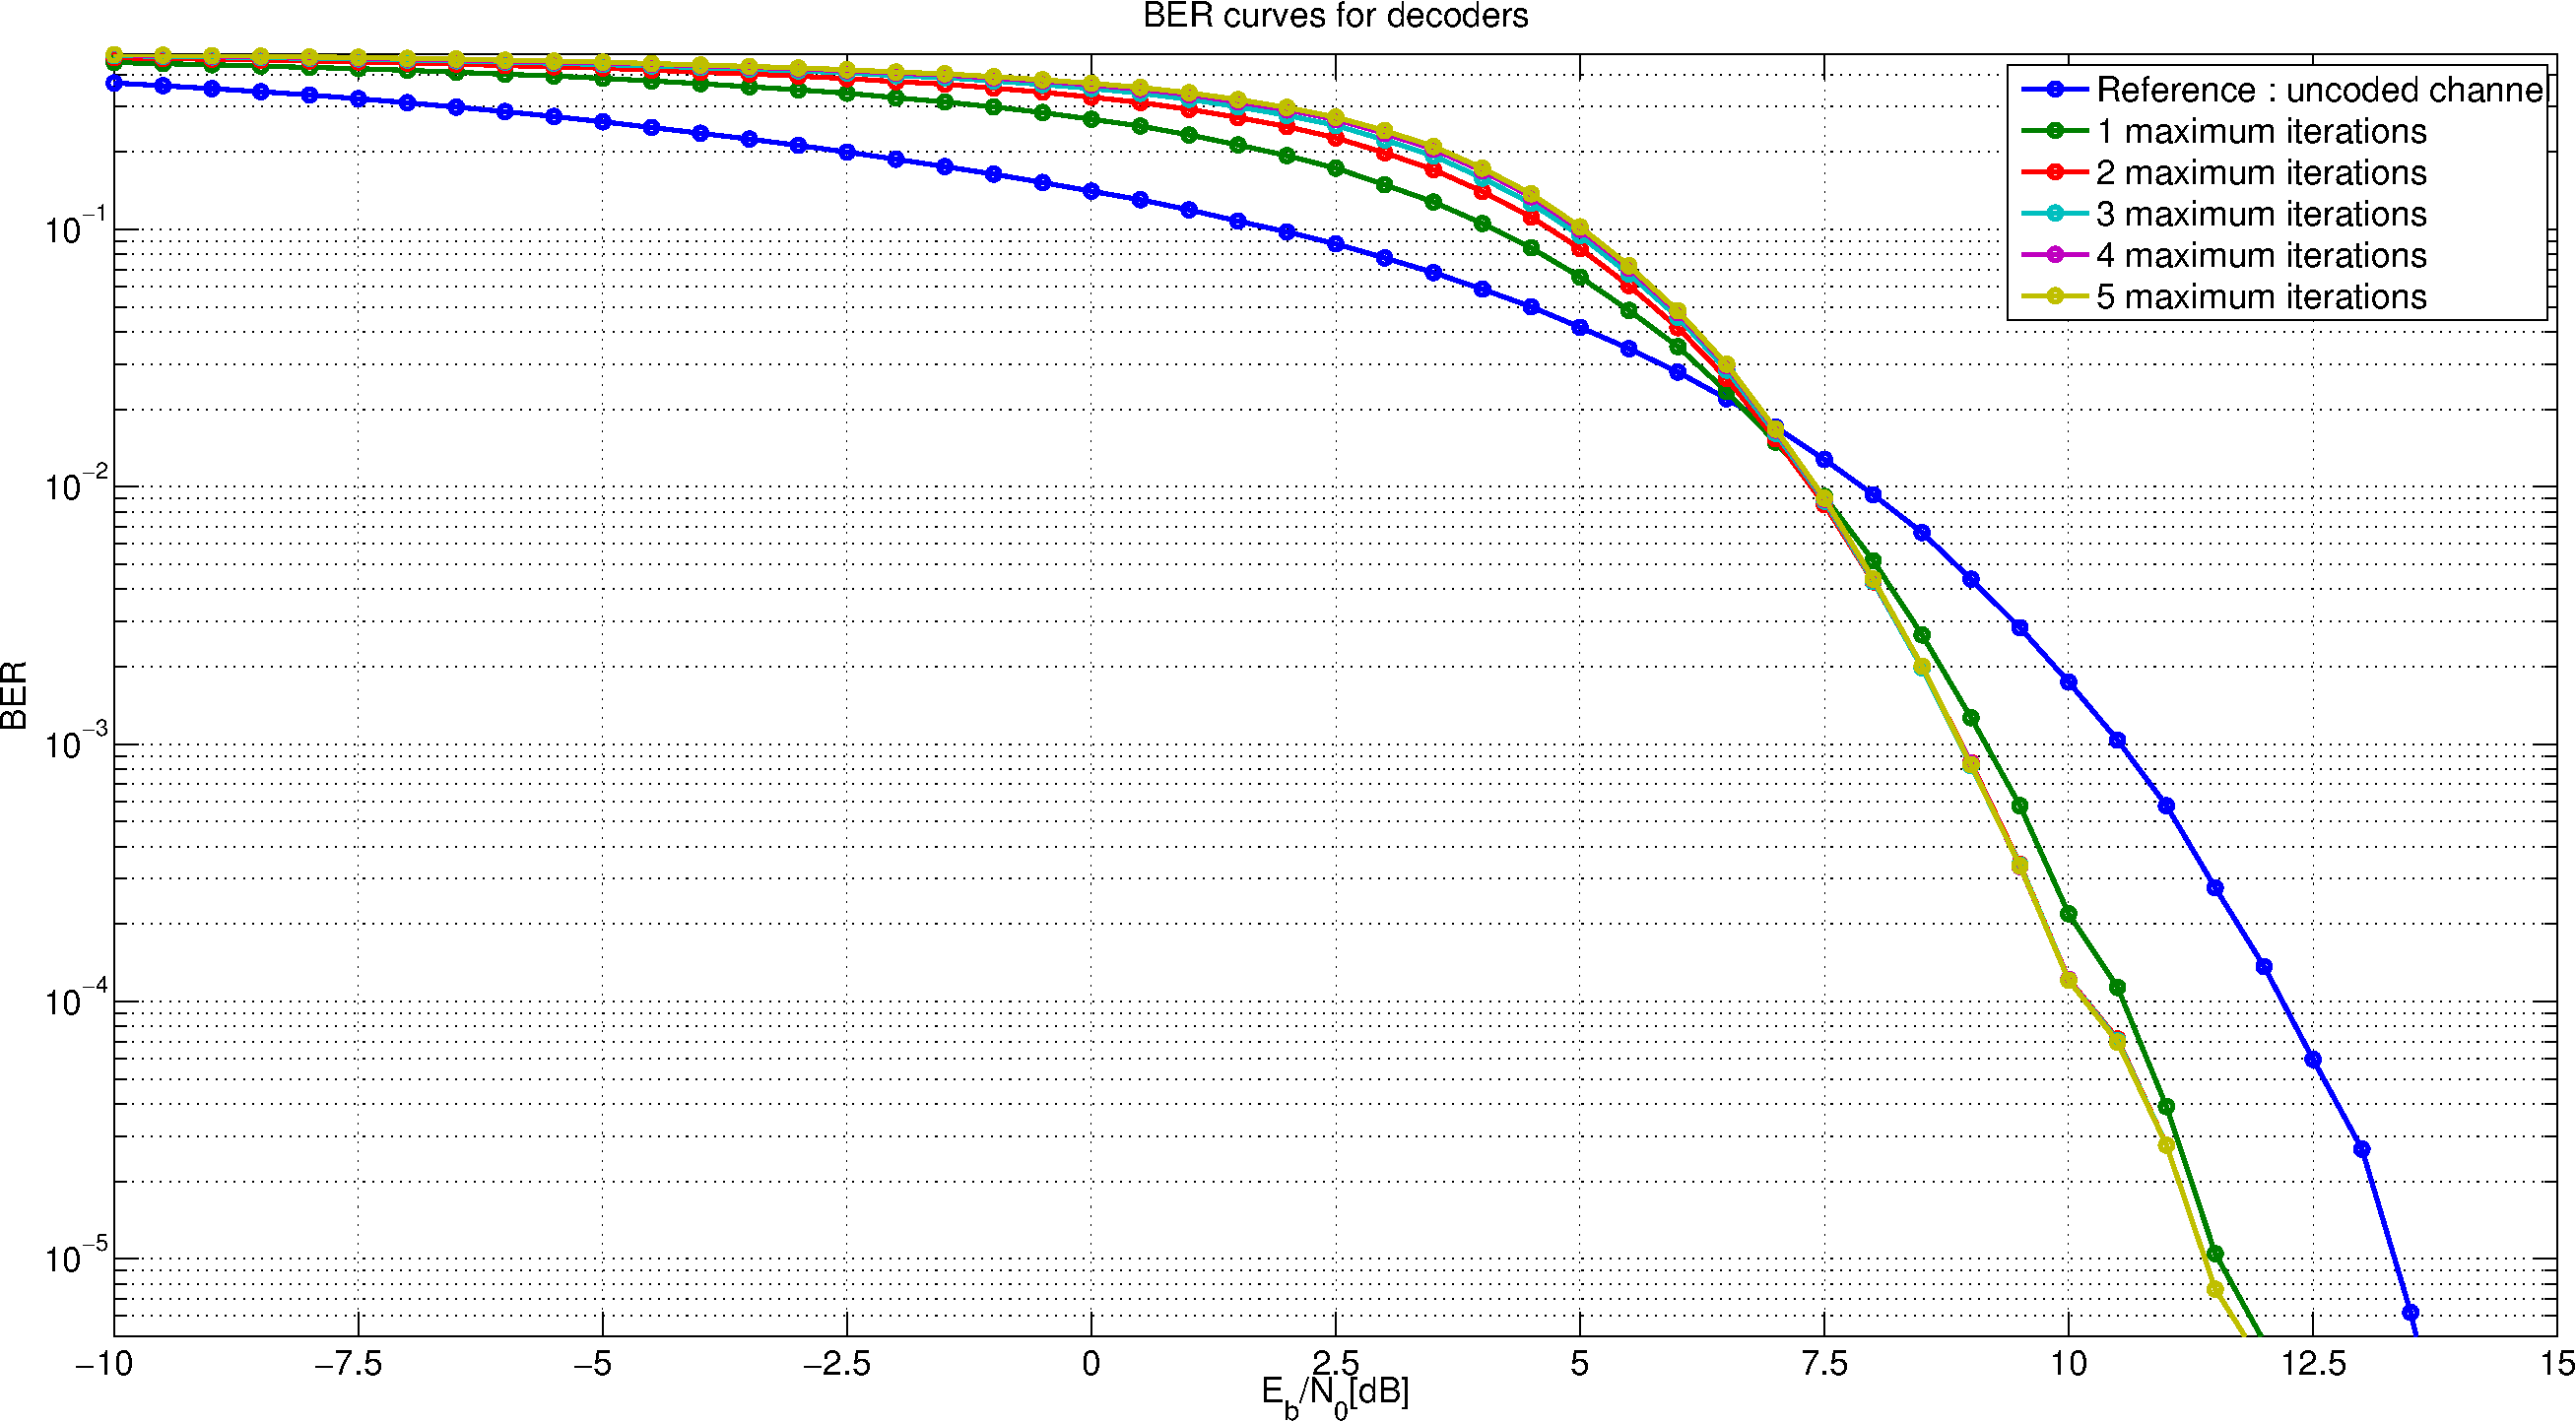
\includegraphics[width=\textwidth]{ldpcBER4.pdf}
    \caption{BER curves for different number of hard decoding iterations, compared with previous results.\label{fig:ldpcBER}}
\end{figure}

\subsection{Soft decoding}
Figure~\ref{fig:sldpcBER} compares the BER curves for the channel without coding, with coding and hard decoding and with different number of soft decoding iterations.
\begin{figure}[htbp]
    \centering
    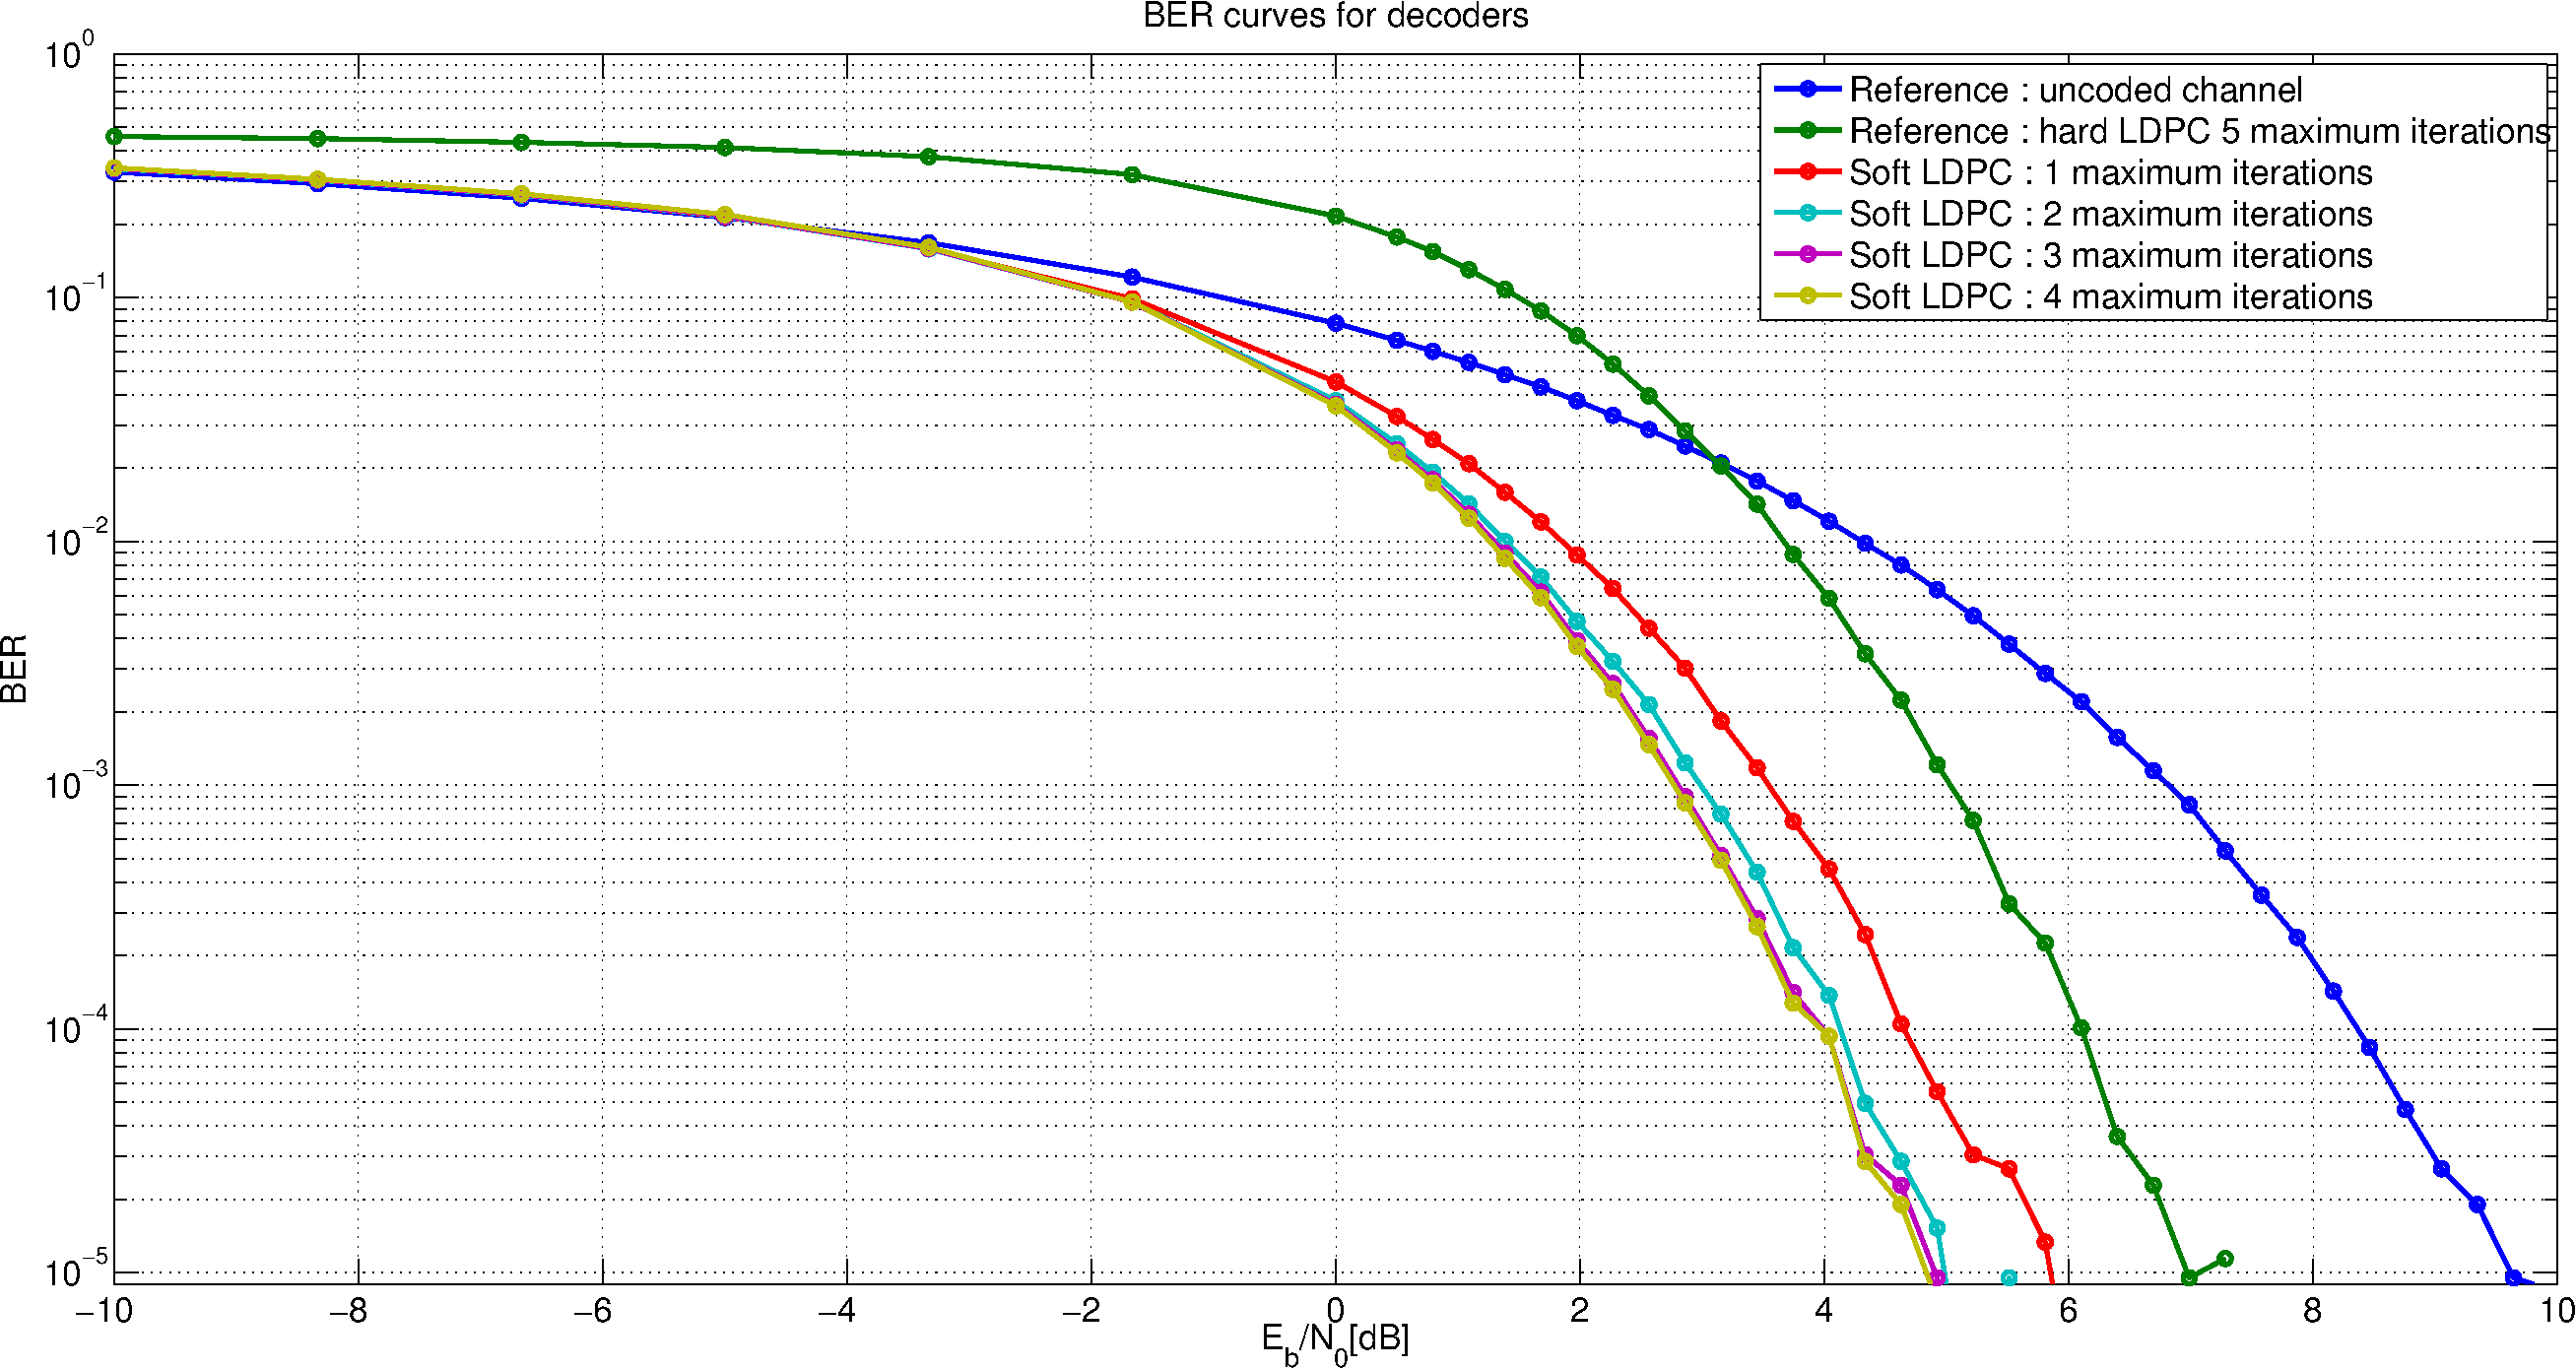
\includegraphics[width=\textwidth]{sldpcBER5.pdf}
    \caption{BER curves for different number of soft decoding iterations, compared with hard decoding and no coding.\label{fig:sldpcBER}}
\end{figure}
As will be explained in the next subsection, BPSK is used for this experiment.
